\documentclass[10pt]{article}

\usepackage[utf8]{inputenc}
\usepackage{amsmath,amsthm,amssymb}
\usepackage{mathrsfs}
\usepackage{amsmath}
\usepackage{epsfig}
\usepackage{color}
\usepackage{indentfirst}
\usepackage{enumitem}
\usepackage[marginparwidth=1in]{geometry}
\usepackage{marginnote}
\usepackage{listings}
\usepackage{xcolor}
\usepackage{graphicx}
\usepackage{latexsym,amsfonts,amssymb,amsthm,amsmath}
\usepackage{hyperref}
\usepackage{cleveref}
\usepackage{matlab-prettifier}
\usepackage[
    backend=biber,
    style=alphabetic,
    sorting=ynt
]{biblatex}
\addbibresource{Reference.bib}

\newenvironment{theorem}[2][Theorem]{
    \begin{trivlist}
\item[\hskip \labelsep {\bfseries #1}\hskip \labelsep {\bfseries #2.}]}{
\end{trivlist}}
\newenvironment{lemma}[2][Lemma]{
    \begin{trivlist}
\item[\hskip \labelsep {\bfseries #1}\hskip \labelsep {\bfseries #2.}]}{
\end{trivlist}}
\newenvironment{exercise}[2][Exercise]{
    \begin{trivlist}
\item[\hskip \labelsep {\bfseries #1}\hskip \labelsep {\bfseries #2.}]}{
\end{trivlist}}
\newenvironment{problem}[2][Problem]{
    \begin{trivlist}
\item[\hskip \labelsep {\bfseries #1}\hskip \labelsep {\bfseries #2.}]}{
\end{trivlist}}
\newenvironment{question}[2][Question]{
    \begin{trivlist}
\item[\hskip \labelsep {\bfseries #1}\hskip \labelsep {\bfseries #2.}]}{
\end{trivlist}}
\newenvironment{corollary}[2][Corollary]{
    \begin{trivlist}
\item[\hskip \labelsep {\bfseries #1}\hskip \labelsep {\bfseries #2.}]}{
\end{trivlist}}

\newlist{indentlist}{enumerate}{2}
\setlist[indentlist, 1]{label=(\alph*), listparindent=\parindent}
\setlist[indentlist, 2]{label=\roman*., listparindent=\parindent}

\newlist{noindentlist}{enumerate}{2}
\setlist[noindentlist, 1]{label=(\alph*), listparindent=\parindent, leftmargin=6mm}
\setlist[noindentlist, 2]{label=\roman*., listparindent=\parindent}

\newenvironment{solution}{
\begin{proof}[Solution]}{
\end{proof}}

\newcommand{\rank}{{\rm rank\;}}
\newcommand{\image}{{\rm Im\;}}
\newcommand{\stack}{{\rm stack\;}}
\newcommand{\Span}{{\rm span\;}}
\newcommand{\diag}{{\rm diag\;}}
\newcommand{\col}{{\rm col\;}}
\newcommand{\cp}{{\rm cp\;}}
\newcommand{\R}{\mathbb{R}}
\newcommand{\N}{\mathbb{N}}
\newcommand{\Z}{\mathbb{Z}}
\newcommand{\Q}{\mathbb{Q}}
\theoremstyle{definition}
\newtheorem{remark}{Remark}
\newtheorem{proposition}{Proposition}
\newtheorem{property}{Property}
\newtheorem{conjecture}{Conjecture}
\newtheorem{assumption}{Assumption}
\newtheorem{example}{Example}
\newtheorem*{examplenull}{Example}
\newtheorem{definition}{Definition}
\newtheorem{fact}{Fact}
\newtheorem{exmp}{Example}[section]
\newtheorem{defn}{Definition}[section]
\def\n{{\bf n}}
\def\m{{\bf m}}
\def\r{{\bf r}}
\def\c{{\bf c}}
\def\scr#1{{\mathcal #1}}
\def\rep#1{(\ref{#1})}
\def\eq#1{
    \begin{equation}#1
\end{equation}}
\def\qed{ \rule{.1in}{.1in}}

\def\matt#1{
    \begin{bmatrix}#1
\end{bmatrix}}
\newcommand{\vecb}[1]{\boldsymbol{#1}}
\newcommand{\dvecb}[1]{\dot{\boldsymbol{#1}}}
\newcommand{\ddvecb}[1]{\ddot{\boldsymbol{#1}}}
\newcommand{\unitv}[1]{\hat{\boldsymbol{#1}}}
\newcommand{\vecbt}[1]{\Tilde{\boldsymbol{#1}}}
\newcommand{\vecbb}[1]{\Bar{\boldsymbol{#1}}}
\newcommand{\norm}[2]{\left\Vert {#1} \right\Vert_{#2}}
\newcommand{\tbf}[1]{\textbf{#1}}
\newenvironment{aequation}
{
    \begin{equation}
    \begin{aligned}}
        {
        \end{aligned}
\end{equation}}

\definecolor{codegreen}{rgb}{0,0.6,0}
\definecolor{codegray}{rgb}{0.5,0.5,0.5}
\definecolor{codepurple}{rgb}{0.58,0,0.82}
\definecolor{backcolour}{rgb}{0.95,0.95,0.92}
\lstdefinestyle{mystyle}{
    backgroundcolor=\color{backcolour},
    commentstyle=\color{codegreen},
    keywordstyle=\color{magenta},
    numberstyle=\tiny\color{codegray},
    stringstyle=\color{codepurple},
    basicstyle=\ttfamily\footnotesize,
    breakatwhitespace=false,
    breaklines=true,
    captionpos=b,
    keepspaces=true,
    numbers=left,
    numbersep=5pt,
    showspaces=false,
    showstringspaces=false,
    showtabs=false,
    tabsize=2,
}
\lstset{style=mystyle}

\begin{document}

% --------------------------------------------------------------
%                         Start here
% --------------------------------------------------------------

\title{Chapter 1 - Sets}
\author{Joseph Le}

\maketitle

\section{Introduction to Sets}

A \textbf{set} is a collection of \textbf{elements}, elements can be anything (numbers, points, functions, etc.). An \textbf{infinite} has an infinite number of elements, otherwise it is a \textbf{finite} set. Two sets are \textbf{equal} if they contain the same elements.

An element $a$ is represented as being \textbf{in} a set $A$ by $a \in A$ and an element $b$ is \textbf{not in} $A$ is shown as $b \notin A$

The set of \textbf{natural numbers}, the set of \textbf{integers}, and the \textbf{rational numbers} have reserved symbols

$$ \mathbb N = \{ 1,2,3,4,5,...\} $$

$$ \mathbb Z = \{ 0, \pm 1, \pm 2, \pm 3, ... \} $$

$$ \mathbb Q = \{ x : x = \frac{m}{n}, \text{ where } m,n \in \Z \text{ and } n \neq 0 \} $$

\noindent as well as the set of \textbf{real numbers}, $\mathbb R$.

For finite sets, the \textbf{cardinality} or \textbf{size} is the number of elements and is denoted as $|A|$, not to be confused with the absolute value of a number, this notation is used only for sets.

The \textbf{empty set} is unique and is a set with no elements usually denoted as $\varnothing$, $\varnothing$, or $\{\}$ and $|\varnothing| = 0$. A set containing the empty set is not empty as $M = {\varnothing}$ contains the empty set, and thus has a cardinality of 1. An analogy often used is thinking of sets as boxes containing things, these things can be other boxes, whether empty or not.

\textbf{Set-builder notation} is a special type of notation used to describe sets by giving its elements rules. Consider the even integers, it can be written as $E = \{0, \pm 2, \pm 4, \pm 6,...\} = \{2n: n \in \mathbb Z\} = \{ n : n \text{ is an even integer} \}= \{ n : n = 2k, k \in \Z \}$. The general format is $X = \{ \text{expression} : \text{rule} \}$

\begin{example}
    Examples of set-builder notation
    \begin{enumerate}
        \item $\{ n : n \text{ is a prime number} \}$
        \item $\{ n^2 : n \in \Z\} = \{ 0, 1, 4, 9, 16, \dots \}$
        \item $\{x \ in \R: x^2-2=0\}=\{ \pm \sqrt{2} \}$
    \end{enumerate}
\end{example}

\begin{example}
    Describe the set $A = \{ 7a + 3b: a,b \in \Z \}$

    \noindent \textbf{Solution:} $A$ contains all numbers of the form $7a + 3b$ where $a$ and $b$ are integers, for example $(a,b) = (0,0) \rightarrow 0$, etc. It can be determined that $A$ only contains integers, but which ones? Suppose $n \in \Z$, and $n = 7n + 3(-2n)$. Here $a = n$ and $b = -2n$, therefore $n \in A$, thus every integer is in $A$ and $A = \Z$.
\end{example}

Intervals on the number line are sets as well, for the real number line, these sets are infinite in size. These sets are given as any two numbers $a,b\in \R$ with $a<b$.

\begin{examplenull}
    These are examples of intervals
    \begin{itemize}
        \item Closed interval: $[a,b] = \{x \in \R : a \leq x \leq b\}$
        \item Open interval: $(a,b) = \{x \in \R : a < x < b\}$
        \item Half-open interval:
            \begin{itemize}
                \item $(a,b] = \{x \in \R : a < x \leq b\}$
                \item $[a,b) = \{x \in \R : a \leq x < b\}$
            \end{itemize}
        \item Infinite interval:
            \begin{itemize}
                \item $(a,\infty) = \{x \in \R: a < x\}$
                \item $[a,\infty) = \{x \in \R: a \leq x\}$
                \item $(-\infty,b) = \{x \in \R: x < b\}$
                \item $(-\infty,b] = \{x \in \R: x \leq b\}$
            \end{itemize}
    \end{itemize}
\end{examplenull}

\subsection*{Exercises}
\begin{enumerate}[label=\Alph*.]
    \item Write each of the following sets by listing their elements between braces
        \begin{enumerate}[label=\arabic*.]
            \item $\{5x-1: x\in\Z\} = \{-16, -11, -6, -1, 4, 9, 15\}$
                \stepcounter{enumii}
            \item $\{x \in \Z : -2\leq x < 7\} = \{-2, -1, 0, 1,2,3,4,5,6\}$
                \stepcounter{enumii}
            \item $\{x \in \R : x^2 = 3\} = \{\pm\sqrt{3}\}$
                \stepcounter{enumii}
            \item $\{x \in \R : x^2+5x=-6\}=\{2,3\}$
                \stepcounter{enumii}
            \item $\{x\in\R : \sin{\pi x} = 0\}=\{0,\pm2,\pm3,\pm4,\dots\}=\Z$
                \stepcounter{enumii}
            \item $\{x \in \Z : |x|<5\}=\{0,\pm1,\pm2,\pm3,\pm4\}$
                \stepcounter{enumii}
            \item $\{x\in\Z:|6x|<5\}=\{0\}$
                \stepcounter{enumii}
            \item $\{5a+2b:a,b\in\Z\}=\Z$
                \begin{proof}
                    If $a$ and $b$ are integers, then $5a+2b$ is also an integer since it is simple multiplication and addition. Then if $n = 5a+2b = 5n+2(-2n) = 5n -4n = n$ where $a = n$ and $b = -2n$, then $5a+2b$ can create any integer, thus the set is equal to the set of all integers, $\Z$. (not sure if this is even a valid proof, just copied the proof from example 1.2)
                \end{proof}
        \end{enumerate}
    \item Write each of the following sets in set-builder notation
        \begin{enumerate}[label=\arabic*.]
                \setcounter{enumii}{16}
            \item $\{2,4,8,16,13,64,\dots\} = \{2^x : x \in \N\}$
                \stepcounter{enumii}
            \item $\{\dots, -6,-3,0,3,6,9,12,\dots\} = \{3x: x \in \Z\}$
                \stepcounter{enumii}
            \item $\{0,1,4,9,16,25,36,\dots\}=\{x^2 : x \in \Z \}$
                \stepcounter{enumii}
            \item $\{3,4,5,6,7,8\} = \{x \in N: 2 < x < 9\}$
                \stepcounter{enumii}
            \item $\{\dots,\frac{1}{8},\frac{1}{4},\frac{1}{2},1,2,4,8,\dots\} = \{2^a: a \in \Z\}$
                \stepcounter{enumii}
            \item $\{\dots, -\pi,-\frac{\pi}{2},0,\frac{\pi}{2},\pi,\frac{3\pi}{2},2\pi,\dots\} = \{\frac{a\pi}{2}: a \in \Z \}$
        \end{enumerate}
    \item Find the following cardinalities
        \begin{enumerate}[label=\arabic*.]
                \setcounter{enumii}{28}
            \item $\left| \{\{1\}, \{2,\{3,4\}\},\varnothing\} \right| = 3$
                \stepcounter{enumii}
            \item $\lvert \{\{\{1\},\{2,\{3,4\}\}\varnothing\}\} \rvert = 1 $
                \stepcounter{enumii}
            \item $\lvert \{x \in \Z : |x| < 10\} \rvert = 19$
                \stepcounter{enumii}
            \item $\lvert \{x \in \Z : x^2 < 10\} \rvert = 7$
                \stepcounter{enumii}
            \item $\lvert \{x \in \N : x^2 < 0\} \rvert = 0$
        \end{enumerate}
    \item Sketch the following sets of points in the $x-y$ plane
        \begin{enumerate}[label=\arabic*.]
                \setcounter{enumii}{38}
            \item $\{(x,y) : x \in [1,2],y\in[1,2]\}$
                \stepcounter{enumii}
            \item $\{(x,y):x\in[-1,1],y=1\}$
                \stepcounter{enumii}
            \item $\{(x,y): |x|=2,y\in[0,1]\}$
                \stepcounter{enumii}
            \item $\{(x,y):x,y\in\R,x^2+y^2=1\}$
                \stepcounter{enumii}
            \item $\{(x,y):x,y\in\R,y\geq x^2-1\}$
                \stepcounter{enumii}
            \item $\{(x,x+k):x\in\R,k\in\Z\}$, this generates a set of parallel lines with slope $m=1$, because $(x,y) = (x,x+k) \rightarrow y=x+k$.
                \stepcounter{enumii}
            \item $\{(x,y)\in\R^2:(y-x)(y+x)=0\}$, here, either $(y-x)=0$ or $(y+x)=0$ or both. The first case gives $y=x$ a line through the origin with slope $m=0$, the second case gives $y=-x$ a line through the origin with slope $m=-1$, and when both are zero, this gives the intersection which is the origin.
                \begin{figure}
                    \centering
                    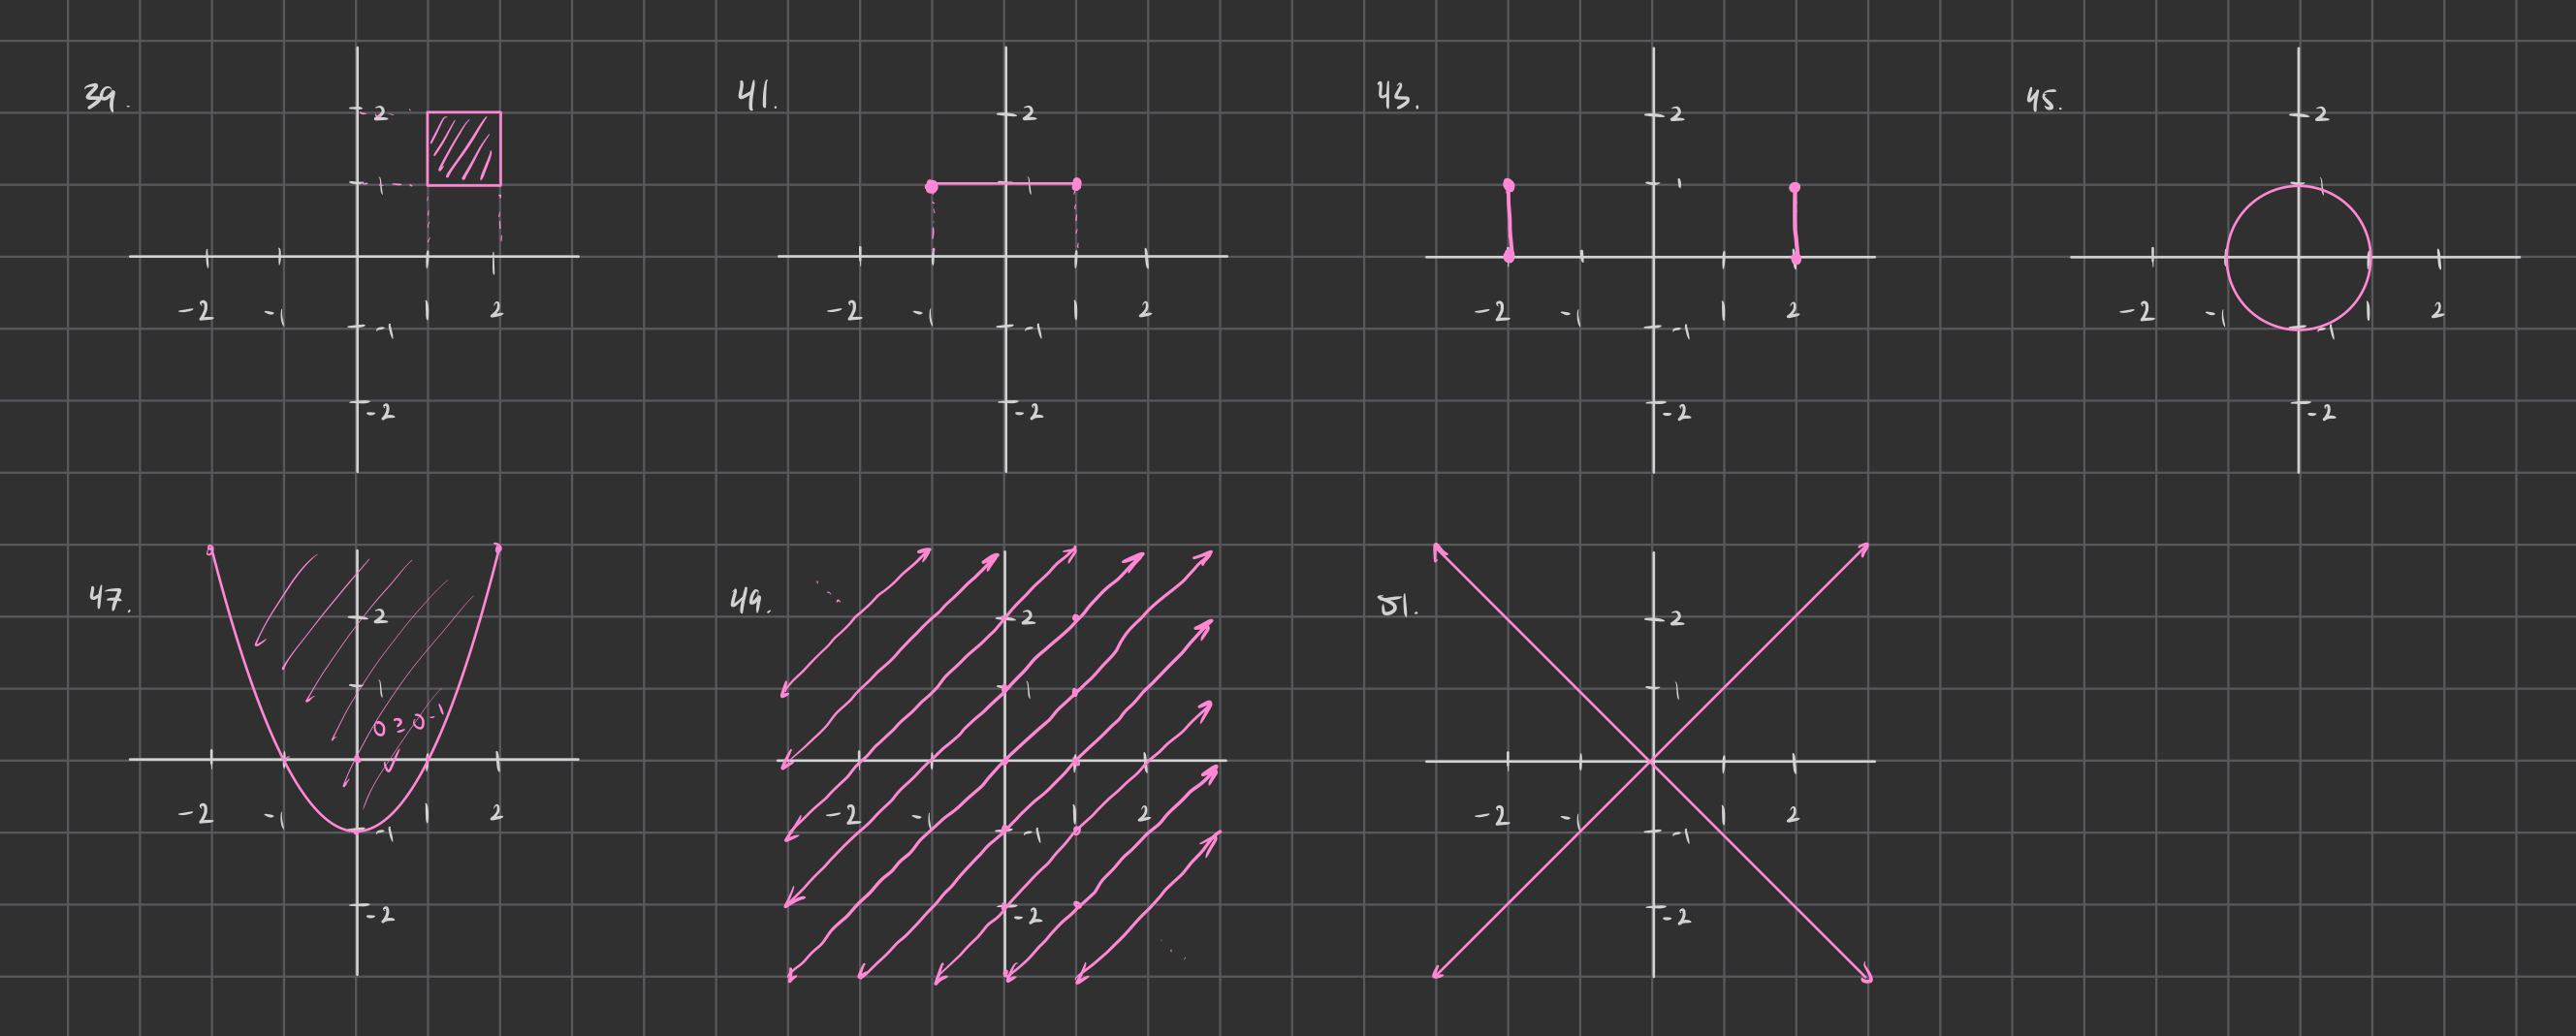
\includegraphics[width=0.75\linewidth]{images/exercise_1_1_D.jpg}
                    \caption{Exercises 1.1.D}
                \end{figure}
        \end{enumerate}
\end{enumerate}

\section{The Cartesian Product}

Given two sets $A$ and $B$, "multiplying" them results a new set denoted as $A\times B$ and is called the \textbf{Cartesian product} of $A$ and $B$.

\begin{definition}
    An \textbf{ordered pair} is a list $(x,y)$ of two elements $x$ and $y$, enclosed in parentheses and separated by a comma.
\end{definition}

For example, $(2,4) \neq (4,2)$ because the order is different even though they contain the same elements. Like sets, the elements don't have to be just numbers.

\begin{definition}
    The \textbf{Cartesian product} of two sets $A$ and $B$ is another set, denoted as $A\times B$ defined as $A \times B = \{ (a,b) : a\in A, b\in B\}$.
\end{definition}

The elements of a Cartesian product are ordered pairs of elements from both sets. For example, if $A = \{k,l,m\}$ and $B = \{q,r\}$, then $A \times B = \{(k,q),(k,r),(l,q),(l,r),(m,q),(m,r)\}$.

\begin{fact}
    \label{cartcard}
    If $A$ and $B$ are finite sets, then $\left| A \times B\right| = \lvert A \rvert \cdot \lvert B \rvert$.
\end{fact}

\begin{example}
    Let $A = \{1,2,3,4,5,6\}$ be the set representing the sides of a dice. $|A \times A| = 6 \cdot 6 = 36$ by Fact \ref{cartcard}. The set $A \times A$ can be thought of the set of possible outcomes of rolling two dice, each result being an ordered pair.
\end{example}

$\R \times \R = \{(x,y):x,y\in \R\}$ is the set of points on the Cartesian plane. $\R \times \N$ is a set of points on lines parallel to the origin whose heights are natural numbers. $\N \times \N$ is the set of points on the Cartesian plane whose coordinates are only natural numbers (in the first quadrant).

Cartesian products can be made with other Cartesian products as well, for example $\R \times (\N \times \Z) = \{(x,(y,z)): x\in\R,(y,z)\in \N \times \Z\}$. \textbf{Ordered triples} are ordered lists of three elements, i.e. $(x,y,z)$. This can be extended to higher numbers as well, i.e. $A_1 \times A_2 \times A_3 \times \cdots \times A_n = \{x_1, x_2, x_3, \dots, x_n: x_i \in A_i \, \forall i \in \N\}$. A \textbf{Cartesian power} is repeated Cartesian products of a set with itself $n$ times ($n > 0 \in \Z$) and is denoted as $A_n = A \times A \times \cdots \times A = \{(x_1,x_2,\dots,x_n): x_i \in A\}$.

\begin{example}
    $S = \{H, T\}$ represents two sides of a coin. Tossing the coin 7 times can be represented with a Cartesian power $S^7$. An element may look like $(H,T,H,H,H,H,T)$. The cardinality of $\lvert S^7\rvert = 2^7$ as there are two options in seven places.
\end{example}

\subsection*{Exercises}
\begin{enumerate}[label=\Alph*.]
    \item Write out the indicated sets by listing their elements between braces.
        \begin{enumerate}[label=\arabic*.]
            \item Suppose $A = \{1,2,3,4\}$ and $B = \{a,c\}$
                \begin{enumerate}[label=(\alph*)]
                    \item $A \times B = \{(1,a),(1,c),(2,a),(2,c),(3,a),(3,c),(4,a),(4,c)\}$
                    \item $B \times A = \{(a,1),(a,2),(a,3),(a,4),(c,1),(c,2),(c,3),(c,4)\}$
                    \item $A \times A = \{
                            \begin{aligned}(1,1),(1,2),(1,3),(1,4),(2,1),(2,2),(2,3),(2,4),
                            \\(3,1),(3,2),(3,3),(3,4),(4,1),(4,2),(4,3),(4,4) \}
                        \end{aligned} $
                    \item $B \times B = \{(a,a),(a,c),(c,a),(c,c)\}$
                    \item $\varnothing \times B = \varnothing$
                    \item $(A\times B)\times B =
                        \begin{aligned}[t]
                            \{ &( (1,a), a),( ( 1,c ), a),( (2,a), a),( (2,c), a), \\
                                &( (3,a), a),( (3,c), a),( (4,a), a),( (4,c), a), \\
                                &( (1,a), c),( ( 1,c ), c),( (2,a), c),( (2,c), c),\\
                            &( (3,a), c),( (3,c), c),( (4,a), c),( (4,c), c) \}
                        \end{aligned} $
                    \item $A \times (B \times B) =
                        \begin{aligned}[t]
                            \{&(1,(a,a)),(1,(a,c)),(1,(c,a)),(1,(c,c)),\\
                                &(2,(a,a)),(2,(a,c)),(2,(c,a)),(2,(c,c)),\\
                                &(3,(a,a)),(3,(a,c)),(3,(c,a)),(3,(c,c)),\\
                            &(4,(a,a)),(4,(a,c)),(4,(c,a)),(4,(c,c))\}
                        \end{aligned}$
                    \item $B^3 =
                        \begin{aligned}[t]
                            \{ (a,a,a),(a,a,c),(a,c,c),(c,c,c),(c,a,a),(c,c,a),(a,c,a),(c,a,c) \}
                        \end{aligned}$
                \end{enumerate}
                \stepcounter{enumii}
            \item
                $
                \begin{aligned}[t]
                    \{x \in \R : x^2 = 2\} \times \{a,c,e\}  &= \{-\sqrt{2}, \sqrt{2}\} \times \{a,c,e\} \\
                    &= \{(-\sqrt{2},a),(-\sqrt{2},c),(-\sqrt{2},e),(\sqrt{2},a),(\sqrt{2},c),(\sqrt{2},e)\}
                \end{aligned}
                $
                \stepcounter{enumii}
            \item
                $
                \begin{aligned}[t]
                    \{x\in\R:x^2=2\}\times\{x\in\R:|x|=2\}  &= \{-\sqrt{2},\sqrt{2}\}\times\{-2,2\} \\
                    &= \{(-\sqrt{2},-2),(-\sqrt{2},2),(\sqrt{2},-2),(\sqrt{2},2)\}
                \end{aligned}
                $
                \stepcounter{enumii}
            \item
                $
                \begin{aligned}[t]
                    \{\varnothing\} \times \{0,\varnothing\} \times \{0,1\} &= \{(\varnothing, 0, 0),(\varnothing,\varnothing,0),(\varnothing,0,1),(\varnothing,\varnothing,1)\}
                \end{aligned}
                $
                \stepcounter{enumii}
        \end{enumerate}
    \item Sketch these Cartesian products on the $x-y$ plane $\R^2$ and $\R^3$.
        \begin{enumerate}[label=\arabic*.]
                \setcounter{enumii}{8}
            \item $\{1,2,3\} \times \{-1,0,1\}$
                \stepcounter{enumii}
            \item $[0,1]\times[0,1]$
                \stepcounter{enumii}
            \item $\{1,1.5,2\}\times[1,2]$
                \stepcounter{enumii}
            \item $\{1\}\times[0,1]$
                \stepcounter{enumii}
            \item $\N \times \Z$
                \stepcounter{enumii}
            \item $[0,1]\times[0,1]\times[0,1]$
                \begin{figure}
                    \centering
                    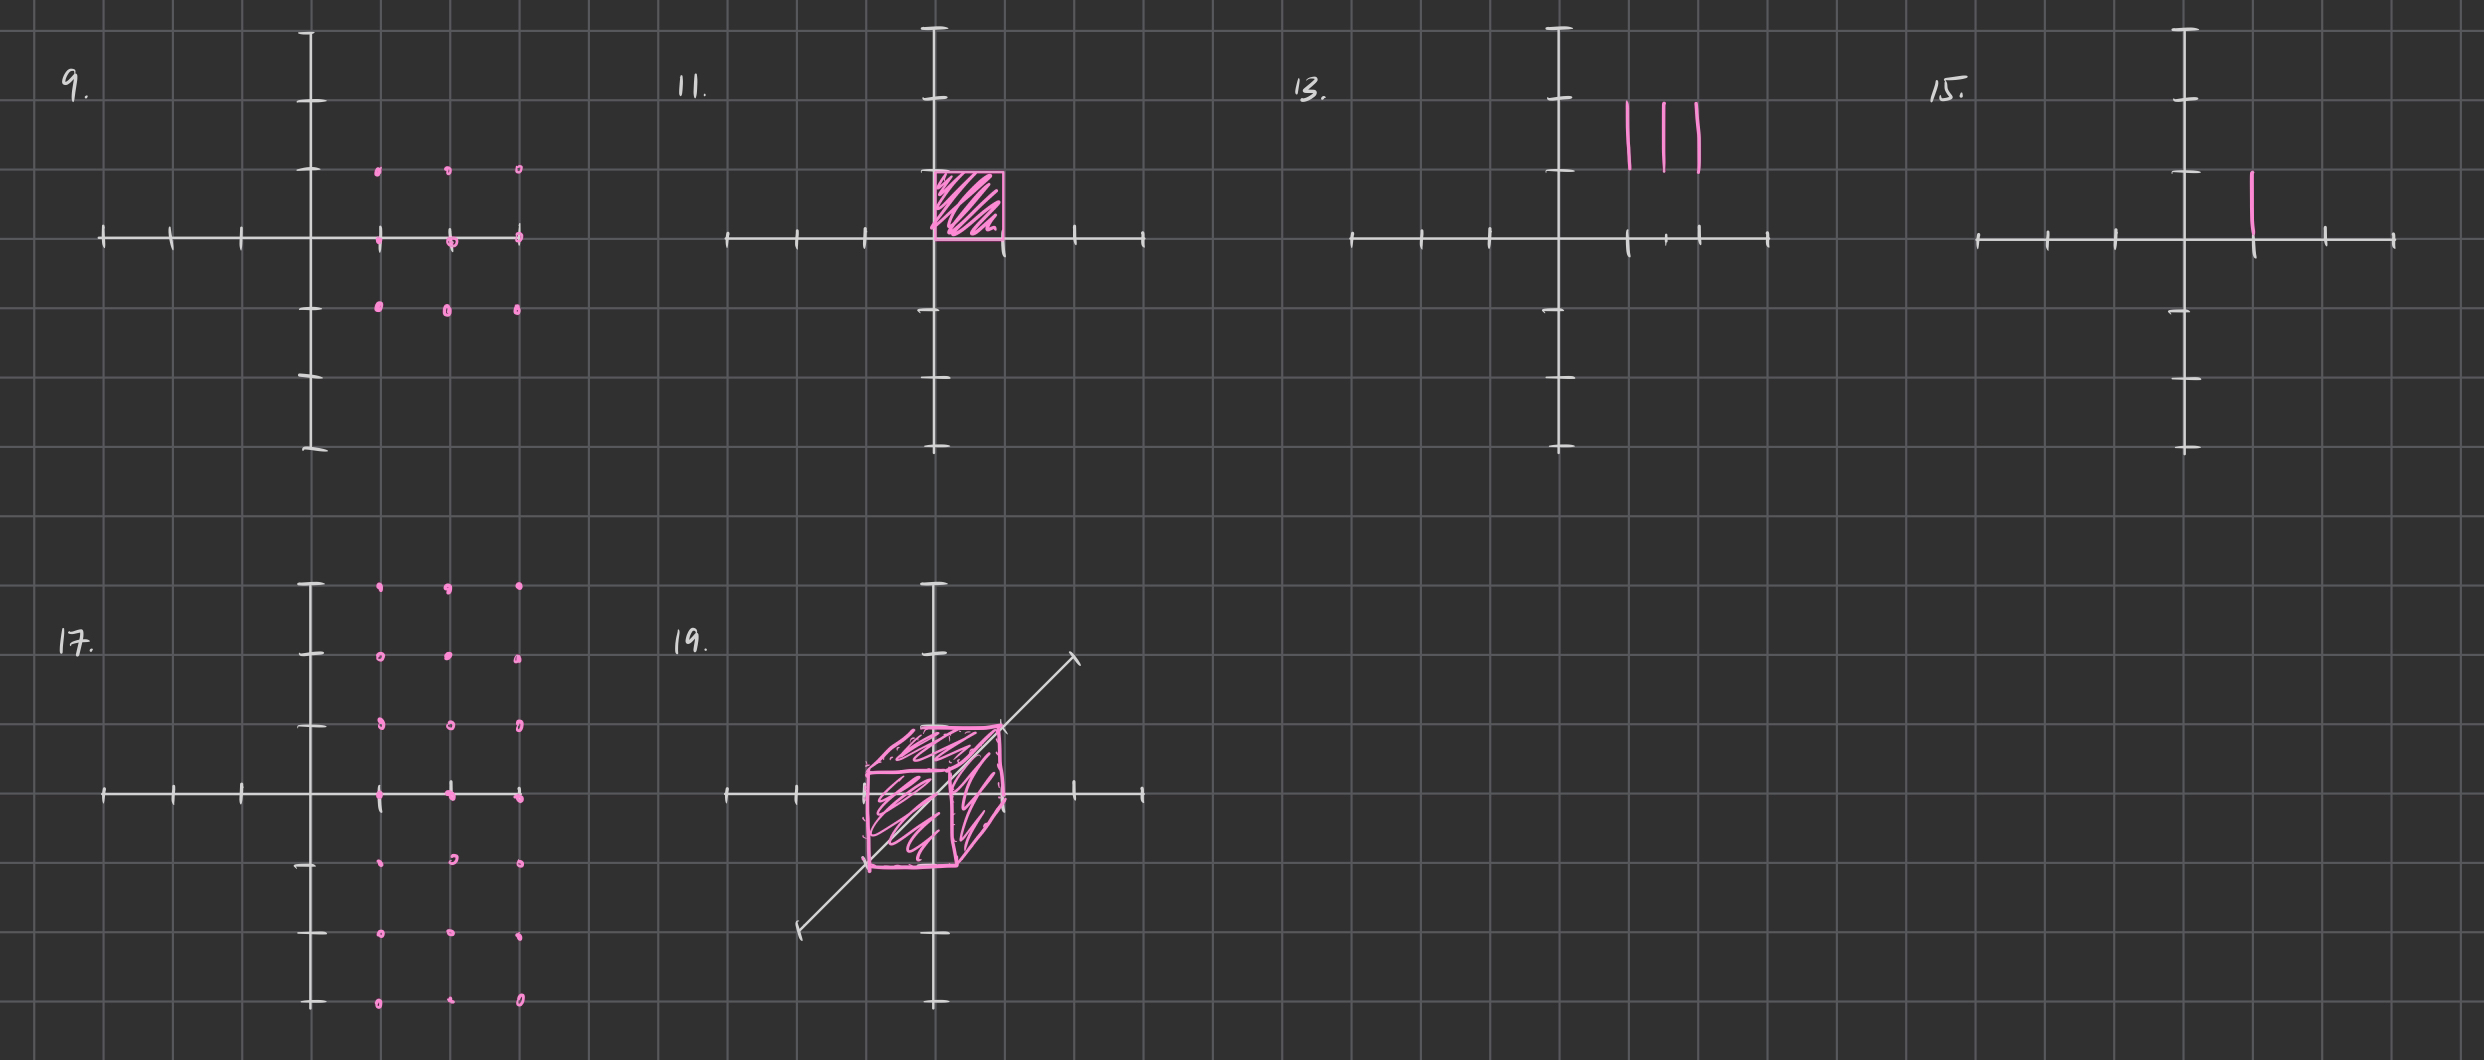
\includegraphics[width=0.75\linewidth]{images/exercise_1_2_B.jpg}
                    \caption{Exercises 1.2.B}
                \end{figure}
        \end{enumerate}
\end{enumerate}

\section{Subsets}
\begin{definition}
    If $A$ and $B$ are sets, and every element of $A$ is in $B$, then $A$ is a \textbf{subset} of $B$ and is denoted as $A \subseteq B$. Otherwise, $A \not\subseteq B$ if $A$ is \textit{not} a subset of $B$ which means that at least one element of $A$ is not an element of $B$
\end{definition}

\begin{example} These are all true
    \begin{enumerate}
        \item $\{2,3,7\} \subseteq \{2,3,4,5,6,7\}$
        \item $\{2,3,7\} \not\subseteq \{2,4,5,6,7\}$
        \item $\{2,3,7\} \subseteq \{2,3,7\}$
        \item $\{(x,\sin{x}: x\in\R\} \subseteq \R^2$
            \item $\{1,3,5,7,9,11,13,17,\dots\} \subseteq \N$
            \item $\N \subseteq \Z \subseteq \Q \subseteq \R$
            \item $\R \times \N \subseteq \R \times \R$
            \item $A \subseteq A, \; \forall A$
            \item $\varnothing \subseteq \varnothing$
        \end{enumerate}
    \end{example}

    The empty set $\varnothing$ is a subset of \textit{all} sets. This is because there are no elements in $\varnothing$ so there is not an element in $\varnothing$ that is not in $B$ or any other set. Formally written:

    \begin{fact}
        The empty set is a subset of all sets, that is, $\varnothing \subseteq B$ for any set $B$.
    \end{fact}

    One can make a subset starting with the empty set and adding elements from the target set. This can help with listing the possible subsets of a given set. A tree-like structure can be created with each layer representing an element from the given set with branches created from true or false statements on whether said element is added to the subset, thus results in the following fact:

    \begin{fact}
        If a finite set has $n$ elements ($|B|=n$), then it has $2^n$ subsets.
    \end{fact}

    Note that for a set $B = \{1,2,\{1,3\}\}$, $\{1,3\}$ is not a subset of $B$ because $3 \not\in B$ but $\{1,3\}$ is an \textit{element} of $B$ and $\{\{1,3\}\} \subseteq B$.

    \begin{example}
        These are all true
        \begin{enumerate}[label=\arabic*., leftmargin=*, align=left]
            \item $1 \in \{1, \{1\}\}$ \dotfill 1 is the first element in the set
            \item $1 \not\subseteq \{1,\{1\}\}$ \dotfill 1 is not a set
            \item $\{1\} \in \{1,\{1\}\}$ \dotfill $\{1\}$ is the second element in the set
            \item $\{1\} \subseteq \{1,\{1\}\}$ \dotfill because it is a set that includes the first element
            \item $\{\{1\}\} \not\in \{1,\{1\}\}$ \dotfill because the set does not contain $\{\{1\}\}$
            \item $\{\{1\}\} \subseteq \{1,\{1\}\}$ \dotfill because it is a set that contains the second element
            \item $\N \not\in \N$ \dotfill $\N$ is a set not a number
            \item $\N \subseteq \N$ \dotfill because $X \subseteq X, \; \forall X$
            \item $\varnothing \not\in \N$ \dotfill because $\varnothing$ is not an element of $\N$
            \item $\varnothing \subseteq \N$ \dotfill because $\varnothing$ is a subset of every set
            \item $\N \in \{\N\}$ \dotfill because it is an element of the set
            \item $\N \not\subseteq \{\N\}$ \dotfill because the elements of $\N$ is not in $\{\N\}$
            \item $\varnothing \not\in \{\N\}$ \dotfill because the set does not contain the empty set
            \item $\varnothing \subseteq \{\N\}$ \dotfill because $\varnothing$ is a subset of every set
            \item $\varnothing \in \{\varnothing,\N\}$ \dotfill because it is the first element in the set
            \item $\varnothing \subseteq \{\varnothing,\N\}$ \dotfill because $\varnothing$ is a subset of every set
            \item $\{\N\} \subseteq \{\varnothing,\N\}$ \dotfill because it is a set containing the second element
            \item $\{\N\} \not\subseteq \{\varnothing,\{\N\}\}$ \dotfill because $\N \not\in \{\varnothing,\{\N\}\}$
            \item $\{\N\} \in \{\varnothing,\{\N\}\}$ \dotfill because $\{\N\}$ is the second element of the set
            \item $\{(1,2),(2,2),(7,1)\} \subseteq \N\times\N$ \dotfill because the elements are in $\N\times\N$
        \end{enumerate}
    \end{example}

    \subsection{Exercises}
    \begin{enumerate}[label=\Alph*.]
        \item List all subsets of the following sets.
            \begin{enumerate}[label=\arabic*.]
                \item $\{1,2,3,4\}$: $
                    \begin{aligned}[t]
                        &\varnothing,\\
                        &\{1\},\{2\},\{3\},\{4\},\\
                        &\{1,2\},\{1,3\},\{1,4\},\{2,3\},\{2,4\},\{3,4\},\\
                        &\{1,2,3\},\{1,3,4\},\{2,3,4\},\{1,2,4\},\\
                        &\{1,2,3,4\}
                    \end{aligned}
                    $
                    \stepcounter{enumii}
                \item $\{\{\R\}\}$: $\varnothing,\{\{\R\}\}$
                    \stepcounter{enumii}
                \item $\{\varnothing\}$: $\varnothing, \{\varnothing\}$
                    \stepcounter{enumii}
                \item $\{\R,\{\Q,\N\}\}$: $\varnothing, \{\R\}, \{\{\Q,\N\}\}, \{\R,\{\Q,\N\}\}$
            \end{enumerate}
        \item Write out the following sets by listing their elements.
            \begin{enumerate}[label=\arabic*.]
                    \setcounter{enumii}{8}
                \item $\{X: X \subseteq \{3,2,a\}, |X| = 2\} = \{\{3,2\},\{3,a\},\{2,a\}\}$
                    \stepcounter{enumii}
                \item $\{X: X \subseteq \{3,2,a\}, |X| = 4\} = \{\}$
            \end{enumerate}
        \item Decide if the following statements are true or false. Explain.
            \begin{enumerate}[label=\arabic*.]
                    \setcounter{enumii}{12}
                \item $\R^3 \subseteq \R^3$: True, because all sets are subsets of themselves.
                    \stepcounter{enumii}
                \item $\{(x,y)\in\R^2:x-1=0\} \subseteq \{(x,y)\in\R^2: x^2-x=0\}$: True, because $\{(x,y)\in\R^2:x-1=0\} ={(1,y): y\in\R}$ which is a vertical line at $x=1$ and the second set contains that as well as a line at $x=0$.
            \end{enumerate}
    \end{enumerate}

    \section{Power Sets}
    \begin{definition}
        If $A$ is a set, the \textbf{power set} of $A$ is another set, denoted as $\mathscr{P}(A) = \{X: X \subseteq A\}$ and defined to be the set of all subsets of $A$.
    \end{definition}

    For example, if $A = \{1,2,3\}$, then $\mathscr{P}(A) =\{\{\},\{1\},\{2\},\{3\},\{1,2\},\{1,3\},\{2,3\},\{1,2,3\}\}$. Also as mentioned previously,

    \begin{fact}
        If $A$ is a finite set, then $|\mathscr{P}(A)| = 2^{|A|}$
    \end{fact}

    \begin{example}
        Sorry too lazy to copy this down, refer to example 1.7 for examples on the above face.
    \end{example}

    It is possible to list out the power set of finite sets, but obviously infinite sets have infinite subsets and are impossible to list out. The set $\R\times\R=\R^2$ is even larger. Any function $f:\R\rightarrow\R$ is a subset of $\R^2$ and any image on a flat plane can be considered a subset of $\R^2$ as well.

    \subsection*{Exercises}

    \begin{enumerate}[label=\Alph*.]
        \item Write the following sets by listing their elements.
            \begin{enumerate}[label=\arabic*.]
                \item $\mathscr{P}(\{\{a,b\},\{c\}\})=\{\varnothing,\{a,b\},\{c\},\{\{a,b\},\{c\}\}\}$
                    \stepcounter{enumii}
                \item $\mathscr{P}(\{\{\varnothing\},5\})=\{\varnothing,\{\{\varnothing\}\},\{5\},\{\{\varnothing\},5\}\}$
                    \stepcounter{enumii}
                \item $\mathscr{P}(\mathscr{P}(\{2\}))=\mathscr{P}(\{\varnothing,2\})=\{\varnothing,\{\varnothing\},\{2\},\{\varnothing,2\}\}$
                    \stepcounter{enumii}
                \item $
                    \begin{aligned}[t]
                        \mathscr{P}(\{a,b\})\times\mathscr{P}(\{0,1\}) &= \{\varnothing,\{a\},\{b\},\{a,b\}\}\times\{\varnothing,\{0\},\{1\},\{0,1\}\}\\
                        &= \{
                            \begin{aligned}[t]
                                &(\varnothing,\varnothing),(\varnothing,\{0\}),(\varnothing,\{1\}),(\varnothing,\{0,1\}),\\
                                &(\{a\},\varnothing),(\{a\},\{0\}),(\{a\},\{1\}),(\{a\},\{0,1\}),\\
                                &(\{b\},\varnothing),(\{b\},\{0\}),(\{b\},\{1\}),(\{b\},\{0,1\}),\\
                            &(\{a,b\},\varnothing),(\{a,b\},\{0\}),(\{a,b\},\{1\}),(\{a,b\},\{0,1\}) \}
                        \end{aligned}
                    \end{aligned}
                    $
                    \stepcounter{enumii}
                \item $
                    \begin{aligned}[t]
                        \mathscr{P}(\{a,b\}\times\{0\}) &= \mathscr{P}(\{(a,0),(b,0)\}) = \{\varnothing,\{(a,0)\},\{(b,0)\},\{(a,0),(b,0)\}\}
                    \end{aligned}
                    $
                    \stepcounter{enumii}
                \item $
                    \{X\subseteq\mathscr{P}(\{1,2,3\}):|X|\leq 1\} = \{X \subseteq \{\varnothing,\{1\},\{2\},\{3\},\{1,2\},\{1,3\},\{2,3\},\{1,2,3\}\}:|X|\leq 1\} = \{\varnothing,\{\varnothing\},\{\{1\}\},\{\{2\}\},\{\{3\}\},\{\{1,2\}\},\{\{1,3\}\},\{\{2,3\}\},\{\{1,2,3\}\}\}
                    \label{crazyone}
                    $
            \end{enumerate}
        \item Suppose that $|A|=m$ and $|B|=n$. Find the following cardinalities.
            \begin{enumerate}[label=\arabic*.]
                    \setcounter{enumii}{12}
                \item $|\mathscr{P}(\mathscr{P}(\mathscr{P}(A)))| = 2^{2^{2^m}}$
                    \stepcounter{enumii}
                \item $|\mathscr{P}(A\times B)| = 2^{m \cdot n}$
                    \stepcounter{enumii}
                \item $|\{X\in\mathscr{P}(A): |X|\leq 1\}| = m + 1$ (see exercise \ref{crazyone})
                    \stepcounter{enumii}
                \item $
                    \begin{aligned}[t]
                        |\mathscr{P}(\mathscr{P}(\mathscr{P}(A \times \varnothing)))| &= |\mathscr{P}(\mathscr{P}(\mathscr{P}(\varnothing)))| \\
                        &= |\mathscr{P}(\mathscr{P}(\{\varnothing,\{\varnothing\}\}))|\\
                        &= |\mathscr{P}(\{\varnothing,\{\varnothing\},\{\{\varnothing\}\}\})|\\
                        & = |\{\varnothing,\{\varnothing\},\{\{\varnothing\}\},\{\{\{\varnothing\}\}\}\}|\\
                        &= 4
                    \end{aligned}
                    $
            \end{enumerate}
    \end{enumerate}

    \section{Union, Intersection, Difference}

    \section{Complement}

    \section{Venn Diagrams}

    \section{Indexed Sets}

    \section{Sets That Are Number Systems}

    \section{Russell's Paradox}

    % \printbibliography
    \end{document}
